%Advances in robotics have been pushing the boundaries of the
%application of robots to automation. There has been a lot of interest
%in robotic picking in this context\cite{correll2016analysis} and
%significant recent efforts have been made for facing the challenges of
%manipulation and grasping.

\IEEEPARstart{A}{utomation} tasks in industrial and service robotics, such as product packing or sorting, often require sets of objects to be arranged in
specific poses on a planar surface. Efficient and high-quality
single-arm solutions have been proposed for such
setups \cite{193}. The proliferation of robot arms, however, including dual-arm setups, implies that industrial settings can utilize multiple robots in the same workspace (Fig \ref{fig:two_arms}). This work explores a) the benefits of coordinated dual-arm rearrangement versus single-arm, b) the combinatorial challenges involved and c) computationally efficient, high-quality and scalable methods.

%While the benefits seem obvious, even for two arms, the challenge
%lies in examining the combinatorial sub-structure of this integrated
%task and motion planning problem.
 
%The current work focuses on rearrangement problems involving two
%arms.  Compared to the sort of solutions that yield high quality
%single arm solutions to these problems, it will be demonstrated that
%significant solution quality improvements can be made, which
%motivates the need to find effective algorithms that can solve the
%dual-arm rearrangement problem.  We seek to bound the cost of $k$-arm
%manipulation.  Note that $c_t$ may be used to capture distance
%(energy) cost or time cost.

%Due to lying at the confluence of various challenging problem
%domains, namely multi-robot motion planning, object rearrangement
%task planning, and combinatorial search, the problem at hand demands
%closer inspection through these lenses. It is desirable to obtain
%some guarantees about the benefits of using more than one arm, before
%endeavoring to study the problem.

A motivating point is that the coordinated use of multiple arms can
result in significant improvements in efficiency. This arises from the following argument.

% \vspace{-.1in}
\begin{lemma}\label{l:k-arm-lower-bound}
There are classes of tabletop rearrangement problems, where a $k$-arm
($k \ge 2$) solution can be arbitrarily better than the optimal
single-arm one.
% \vspace{-.3in}
\end{lemma}

For instance, assume two arms that have full (overhand) access to a 
unit square planar tabletop. There are $n$ objects on the table, 
divided into two groups of $\frac{n}{2}$ each. Objects in each group 
are $\varepsilon$-close to each other and to their goals. Let the 
distance between the two groups be on the order of $1$, i.e., the two 
groups are at opposite ends of the table. The initial position of each 
end-effector is $\varepsilon$-close to a group of objects. Let the cost 
of each pick and drop action be $c_{pd}$, while moving the 
end-effector costs $c_t$ per unit distance. Then, the $2$-arm 
cost is no more than $2nc_{pd} + 2n\varepsilon c_t $.  A single arm 
solution costs at least $2nc_{pd} + (2n-1)\varepsilon c_t + 
c_t$. If $c_{pd}$ and $\varepsilon$ are sufficiently small, the $2$-arm 
cost can be arbitrarily better than the single-arm one. The argument 
also extends to $k$-arms relative to $(k-1)$-arms.

In most practical setups, the expectation is that a $2$-arm solution
will be close to half the cost (e.g., time-wise) of the single-arm 
case, which is a desirable improvement. While there 
is coordination overhead, the best $2$-arm solution cannot do worse; simply 
let one of the arms carry out the best single arm solution while the 
other remains outside the workspace. More generally:

% \vspace{-.1in}
\begin{lemma}\label{l:2-arm-no-worse}
For any rearrangement problem, the best $k$-arm ($k \ge 2$) solution
cannot be worse than an optimal single arm solution.
% \vspace{-.1in}
\end{lemma}

The above points motivate the development of scalable algorithmic
tools for such dual-arm rearrangement instances. This work considers
certain relaxations to achieve this objective. In particular,
monotone tabletop instances are considered, where the start and goal
object poses do not overlap.  Furthermore, the focus is on
synchronized execution of pick-and-place actions by the two arms. i.e., where the two arms simultaneously transfer (different) objects, or simultaneously move towards picking the next objects.
Theoretical arguments and experimental evaluation indicate that this does not significantly degrade solution
quality.

\begin{figure}[t]
% \vspace{-0.15in}
	\centering
	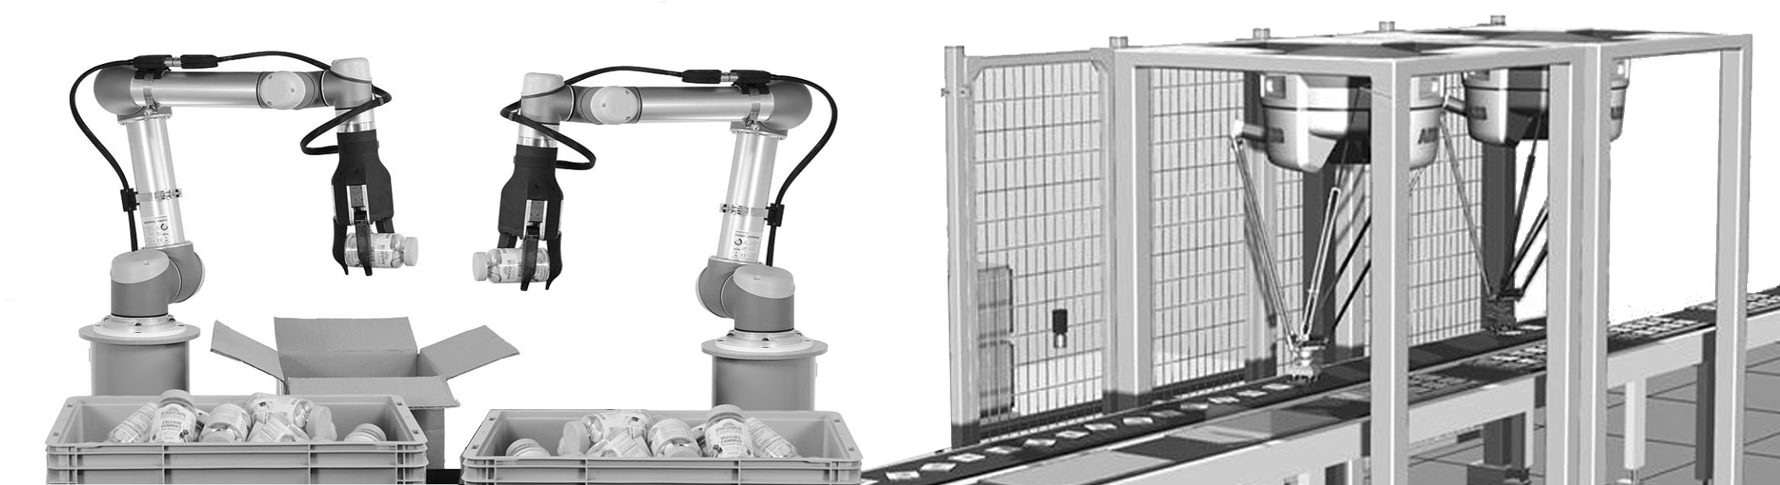
\includegraphics[width=0.48\textwidth]{figures/two_arms}
% 	\vspace{-0.1in}
	\caption{Example of dual-arm setups that can utilize
	algorithms proposed in this work.}
	\label{fig:two_arms}
% 	\vspace{-0.25in}
\end{figure}



The first contribution is the study of the combinatorial structure of
synchronous, monotone dual-arm rearrangement. Then, a mixed integer linear programming (\milp) model is
proposed that achieves optimal coordinated solutions in this domain.
The proposed efficient algorithm {\tt Tour\_Over\_Matching} (\algo) significantly improves in scalability. \algo\ first optimizes the
cost of object transfers and assigns objects to the two arms by
solving an optimal matching problem. It minimizes the cost of
moves from an object's goal to another object's start pose per
arm as a secondary objective by employing a {\tt TSP} solution. Most
of the computation time is spent on the many calls to a
lower-level motion planner that coordinates the two arms. A lazy
evaluation strategy is proposed, where motion plans are evaluated for candidate solution sequences. This results in significant computational improvement and
reduces the calls to the motion planner.  An analysis
studies the expected improvement in solution quality
versus the single arm case, as well as the expected cost overhead from a
synchronous solution.

Finally, experiments for i) a simple planar picker setting, and ii) two 7-DOF Kuka arms, demonstrate a nearly two-fold
improvement against the single arm case for the proposed approach in practice. The algorithm exhibits close to optimal solutions and good scalability. 
The lazy evaluation strategy significantly improves computation costs for both the optimal and proposed methods.

\tase{
The current archival version is an extension of previous work and several additions have been made to the draft to provide a more holistic inspection of the problem, chiefly:
\begin{enumerate}
	\item An additional benchmark has been added to demonstrate the efficacy of the proposed approach in problem domains where all the object positions do not lie in the shared workspace.
	\item It has been argued that smoothing can be used to alleviate the sychronization assumption. Data from the effects of smoothing the solutions in the experiments have been reported and show that the minor improvements highlight that in practice the synchronization assumption is not tragic.
	\item A k-arm extension of the asymptotic cost bound in the asynchronous case has been included.
	\item The proof for the asymptotic cost bound estimate for 2-arms under the synchronization assumption has been expanded, and Monte-Carlo trials have been reported in a simplified setup to validate the analysis model.
\end{enumerate}
}
%The computational costs of both the optimal
%and the proposed method are significantly improved from the lazy
%evaluation strategy. 
% When the synchronous solutions are smoothed to
% asynchronous ones, there is not significance difference in overall
% path quality. \kiril{This statement is unclear. What is the benefit from performing this step?}
